\documentclass[aspectratio=169,dvipsnames,c]{beamer}
\usepackage[T2A]{fontenc}
\usepackage[russian]{babel}
\usepackage{fontawesome5}
\usepackage{xeCJK}
\usepackage{tabularx}

\usepackage[absolute,overlay]{textpos}
\usepackage{pgf-pie}

% Подчёркивания
\usepackage{ulem}
\renewcommand{\ULdepth}{1.0pt}

\newcommand\Insertsubsection{}
\newcommand\Setsubsection[1]{
  \subsection{#1}
  \renewcommand\Insertsubsection{#1}
}

% Гиперссылки
\usepackage{hyperref}
\hypersetup{
  colorlinks=true,
  linkcolor=AccentColor,
  filecolor=AccentColor,
  urlcolor=AccentColor,
}

\newcommand\uhref[2]{{\color{AccentColor} \uline{\href{#1}{#2}}}}

\newcommand\ExampleIcon{{\color{AccentColor} \faFlask}}

\newcommand\ExampleNote{%
  \begin{textblock}{1}(15, 15)
    \ExampleIcon{}
  \end{textblock}
}

\newcommand\subtitlepage[2]{
  \subtitle{#1}
  \section{#1: #2}
  \begin{bg-frame}
    \vspace{1.75\baselineskip}
    {\Huge \insertsubtitle\\}
    \vspace{0.5\baselineskip}
    {\large #2}
  \end{bg-frame}
}

% Включение исходного кода.
\usepackage{minted}
\setminted{%
  breaklines,
  fontsize=\scriptsize,
  frame=leftline,
  linenos,
  showspaces,
  space=\char"22C5,
  spacecolor=Black!40,
  style=friendly, % Стили можно посмотреть командой pygmentize -L styles
}

\usepackage{smartdiagram}
\smartdiagramset{%
  module shape=rectangle,
  border color=Black!80,
  font=\scriptsize,
  text color=White,
  uniform color list=AccentColor for all items
}
\usesmartdiagramlibrary{additions}

% Отключает градиенты в рисунках smartdiagram, может повредить TikZ-графику
\tikzset{module/.append style={top color=\col,bottom color=\col}}
\tikzset{every shadow/.style={fill=none,shadow scale=0}}

\usepackage{shadowtext}
\shadowcolor{Black}
\shadowoffset{0.5pt}

\usetheme{custom}

\graphicspath{{bundled-img/}{img/}{icons/}}
\hypersetup{colorlinks=true}

\usepackage{relsize}

\newcommand\inlineicon[1]{
  {\larger[2] \color{AccentColor} \raisebox{-0.08\baselineskip}{#1}}
}

\newcommand\baselinespace{\vspace{\baselineskip}}

\newlength{\rulewidth}
\setlength{\rulewidth}{0.4pt}

\newcommand\roundpic[3][]{
  \begin{tikzpicture}[#1]
    \node[
      circle,
      minimum width = #2,
      path picture = {
          \node[] at (path picture bounding box.center){
            \includegraphics[width=#2]{#3}};
      }
    ]{};
  \end{tikzpicture}
}

% Requires to build twice to calculate position
\newcommand\overlaypic[3]{
  \begin{tikz}[remember picture, overlay]
    \node[anchor=#1] at (current page.#1) {\includegraphics[#2]{#3}};
  \end{tikz}
}

\newenvironment{Frame}[2][]
{%
  \subsection{#2}

  \begin{frame}[environment=Frame, {#1}]
    \frametitle{#2}
}
{%
  \end{frame}
}

\newenvironment{custom-bg-frame}[1]
  {%
    \begingroup
      \setbeamertemplate{background}{%
        \includegraphics[
          width=\paperwidth,
          height=\paperheight,
          keepaspectratio]{#1}
      }
      \color{White}
      \begin{frame}[c]
      \centering
  }
  {%
      \end{frame}
    \endgroup
  }

\newenvironment{bg-frame}
  { \begin{custom-bg-frame}{background.jpg} }
  { \end{custom-bg-frame} }

\newcommand\liveframe{
  \begin{bg-frame}
    \vspace{36pt}
    {\fontsize{60pt}{\baselineskip}\selectfont \bfseries LIVE}
  \end{bg-frame}
}

\newwrite\tempfile
\immediate\openout\tempfile=slidelist.txt

\newcounter{SlideNumber}
\addtobeamertemplate{frametitle}{}{%
  \stepcounter{SlideNumber}
  \immediate\write\tempfile{%
    \theSlideNumber\space\insertframetitle%
  }
}

\author{Антон Карманов}

\newcommand\insertcontacts{%
  \hypersetup{urlcolor=White}
  \href{%
    mailto:Антон Карманов <a.karmanov@inventati.org>
  }{%
    \faEnvelope{} a.karmanov@inventati.org
  }
}

\newcommand{\homepage}{%
  https://gitlab.com/bergentroll-docs/saltstack-tutorial
}

\newcommand{\inserthomepage}{%
  \hypersetup{urlcolor=White}
  \href{%
    \homepage
  }{%
    \faIcon{git-alt} \homepage{}
  }
}

\newcommand\insertreaderbrief{
  \setbeamertemplate{itemize item}[circle]
  \begin{itemize}
    \item Инженер АО <<Гринатом>>
    \item За свободное ПО
    \item За открытый контент
    \item Люблю выдержанный чай \char"8336
  \end{itemize}
}


\title{Пособие по SaltStack}

\begin{document}

\section{Введение}

\begin{bg-frame}
  \vspace{1.50\baselineskip}
  {\Huge \inserttitle\\}
  \rule{180pt}{\rulewidth}\\
  \insertauthor{} \insertcontacts{}\\
  \vspace{0.25\baselineskip}
  \inserthomepage{}

  \newlength{\blockheight}
  \setlength{\blockheight}{\dimexpr(\textheight)-\baselineskip}
  \begin{textblock*}{\paperwidth} (-1em, \blockheight)
    \tiny \raggedleft{}
    \shadowtext{сборка документа \insertdate{}}
  \end{textblock*}

\end{bg-frame}

\begin{Frame}[t]{Обо мне}
  \begin{columns}[c]
    \begin{column}{0.35\textwidth}
      \begin{figure}
        \roundpic[]{105pt}{snowy}
      \end{figure}
    \end{column}
    \begin{column}{0.65\textwidth}
      {\large \insertauthor{}}
      \baselinespace{}
      \insertreaderbrief{}
    \end{column}
  \end{columns}
\end{Frame}

\begin{Frame}[c]{Структура пособия}
  \centering

  \smartdiagramset{%
    back arrow disabled=true,
    module y sep=40pt,
    font=\scriptsize,
    text width=8em,
  }

  \smartdiagramanimated[flow diagram]{%
    Пара вводных слов,
    Администрирование\\ системы,
    Базовая эксплуатация,
    Углублённые темы
  }
\end{Frame}

\subtitlepage{SaltStack}{Начало}

\begin{Frame}{SaltStack --- это}
  \begin{itemize}[<+-| alert@ +>]
    \item[\faWrench] Система управления конфигурациями\\
    \item[{\faCircle[regular]}] Шина на ZeroMQ\footnote<.->{\url{https://zeromq.org/}}
    \item[\faCubes] Python и модульность
    \item[\faIndent] Профессия YAML-программист
    \item[\faCloud] \relax <<Провиженинг>> для IaaS
    \item[\faCube] В народе --- <<соль>>
  \end{itemize}

  \vfill

  \begin{center}
    
\includegraphics[width=240pt]{saltstack-logo}
  \end{center}

\end{Frame}

\begin{Frame}{Системы управления конфигурациями}

  \setbeamercovered{invisible}

  \centering
  \def\arraystretch{1.5}
  \begin{table}\begin{tabularx}{\textwidth}{r|lp{6em}p{4em}X}
    СУК & Год & На чём & DSL & Особенности \\
    \hline
    \onslide<+->{
      \alert<.>{Puppet} & 2005 & Ruby & Свой & Pull \\
    }
    \onslide<+->{
      \alert<.>{Chef} & 2009 & Ruby, Erlang & Ruby & Pull, веб-интерфейс} \\
    \onslide<+->{
      \alert<.>{\bf SaltStack} & \bf 2011 &
      \bf Python\footnote{Сплошной Python} & \bf YAML & \bf Pull (и Push),
      корп-версия\\
    }
    \onslide<+->{
      \alert<.>{Ansible} & 2012 & Python, Ruby & YAML &
      Push (и Pull), Ansible Tower
    }
  \end{tabularx}\end{table}
\end{Frame}

\liveframe{}

\begin{Frame}{Глоссарий}
  \centering
  \def\arraystretch{1.5}
  \small
  \begin{table}\begin{tabularx}{\textwidth}{l|X|l}
    В SaltStack & Значение & В Ansible \\
    \hline
    Мастер & Сервер & Узел (нода) управления \\
    Миньон & Клиент & Управляемый узел \\
    Формула & Декларативный конфиг клиента & Плейбук\\
    Состояние & Элементарная единица конфига клиента & Таск \\
    Грейн & Переменная, полученная от клиента & Факт \\
    Топ-файл & Маппинг хостов & Инвентарь (хосты)\\
    Пиллары & Устанавливаемая переменная & Инвентарь (переменные) \\
  \end{tabularx}\end{table}
\end{Frame}

\begin{Frame}{Топология}
  \centering
  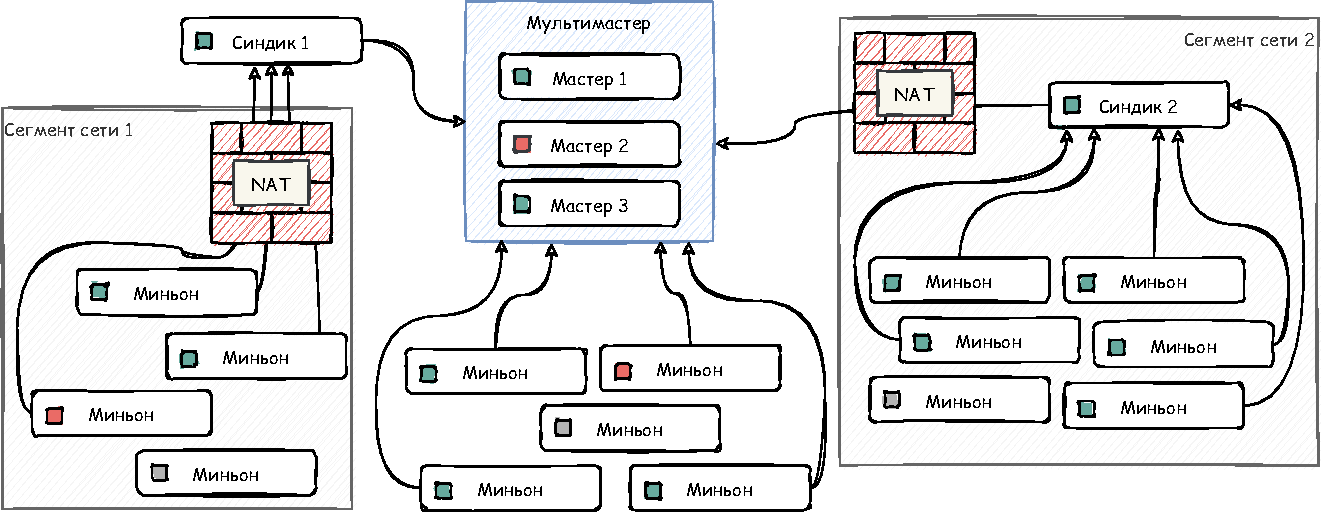
\includegraphics[width=0.95\textwidth]{saltstack-topology}
\end{Frame}

\begin{Frame}{Архитектура}
  \centering
  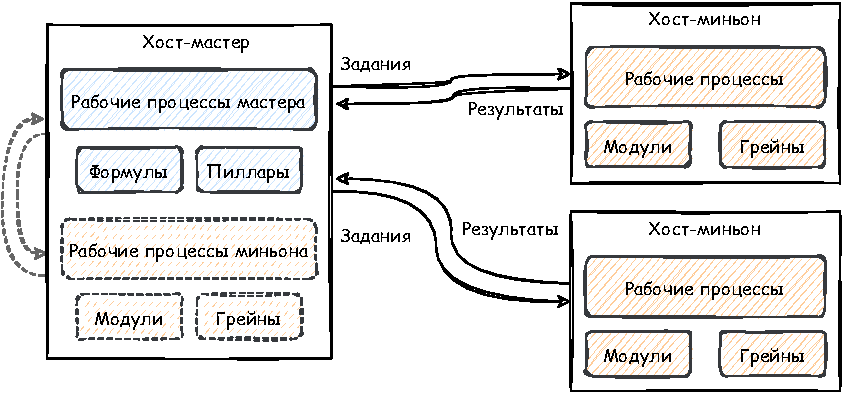
\includegraphics[width=0.80\textwidth]{saltstack-architecture}
\end{Frame}

\begin{Frame}{Данные}
  \begin{columns}
    \begin{column}{0.45\textwidth}
      \begin{itemize}[<+-| alert@ +>]
        \item Grains (<<крупицы соли>>) \baselinespace
        \item Pillars (<<соляные столпы>>) \baselinespace
        \item Salt Mine (<<соляная шахта>>)
      \end{itemize}
    \end{column}
    \begin{column}{0.55\textwidth}
      \includegraphics<1>[width=0.9\textwidth]{grains-photo}
      \includegraphics<2>[width=0.9\textwidth]{salt-pillar}
      \includegraphics<3>[width=0.9\textwidth]{salt-mine-photo}
    \end{column}
  \end{columns}
\end{Frame}

\begin{Frame}{Типы модулей}
  \overlaypic{south east}{width=100pt}{boxes}
  \begin{itemize}[<+-| alert@ +>]
    \item \texttt{salt.modules}
    \item \texttt{salt.states}
    \item \texttt{salt.grains}
    \item \texttt{salt.pillar}
    \item \texttt{salt.renderer}
    \item \ldots
    \item Десятки их!
  \end{itemize}
\end{Frame}

\begin{Frame}{YAML}
  \centering
  \huge У вас найдётся минутка поговорить о ещё одном языке разметки?
\end{Frame}

\begin{frame}{YAML}
  \ExampleNote{}

  \begin{columns}
    \begin{column}{0.5\textwidth}
      \begin{itemize}[<+-| alert@ +>]
        \item Форматирование отступами
        \item Скалярные типы
        \item Мультистрочные литералы\footnotemark{}
        \item Словари и последовательности
        \item Включает в себя JSON
        \item Наследование (на десерт)
      \end{itemize}
    \end{column}

    \begin{column}{0.5\textwidth}
      \inputminted{yaml}{../examples/yaml-file.yaml}
    \end{column}
  \end{columns}

  \onslide<3->\footnotetext{\url{https://yaml-multiline.info}}

\end{frame}


\subtitlepage{SaltStack}{Администрирование}

\begin{Frame}{Установка}

  \only{\overlaypic{south east}{width=80pt}{rocket}}

  \begin{center}
    0.6.0 \dots{} 2018.3.0 $\to$ 2019.2.0 $\to$ 3000 \dots{} \bfseries{3004.1}
  \end{center}

  \vfill

  \pause{}

  \begin{itemize}[<+-| alert@ +>]
    \item Salt Bootstrap\footnote{%
      \url{https://github.com/saltstack/salt-bootstrap}}
    \vfill
    \item Из репозитория дистрибутива
    \vfill
    \item Из репозитория SaltStack\footnote<3->{\url{https://repo.saltproject.io/}}
    \vfill
    \item PyPI: \texttt{pip install salt}
    \vfill
  \end{itemize}
\end{Frame}

\liveframe{}

\begin{Frame}{Конфиг}
  \begin{itemize}
    \item \texttt{/etc/salt/master} \ExampleIcon{}
    \item \texttt{/etc/salt/minion} \ExampleIcon{}
  \end{itemize}

  \vfill
  \pause{}

  \inlineicon{\faInfoCircle} Можно два в одном\only<2>{\dots}
  \pause{} (но не нужно)

  \vfill
  \pause{}

  \begin{block}{В помощь}
    \setbeamertemplate{itemize items}{\faTerminal}
    \small
    \begin{itemize}
      \item \texttt{salt-run fileserver.dir\_list [saltenv=ОКРУЖЕНИЕ]}
      \item \texttt{salt-run fileserver.file\_list [saltenv=ОКРУЖЕНИЕ]}
    \end{itemize}
  \end{block}

\end{Frame}

\begin{Frame}{Пара слов о файлах}
  \begin{itemize}[<+-| alert@ +>]
    \item[\faSync] Конфиг перечитывается в рантайме
    \item[\faFolder] Данные времени исполнения в \texttt{/var/cache/salt/}
  \end{itemize}
\end{Frame}

\begin{Frame}{Запуск}
  \begin{itemize}[<+-| alert@ +>]
    \vfill
    \item \texttt{salt-master} (команда и служба)\vfill
    \item \texttt{salt-minion} (команда и служба)\vfill
    \item[\faBug] Ключ \texttt{--log-level=debug}
    \vfill
  \end{itemize}

\end{Frame}


\subtitlepage{SaltStack}{Эксплуатация}

\begin{Frame}{Команды}

  \overlaypic{south east}{width=80pt}{terminal}

  \begin{itemize}[<+-| alert@ +>]
    \item \texttt{salt-key} \ExampleIcon{}
    \vfill
    \item \texttt{salt ЦЕЛЬ МОДУЛЬ.ФУНКЦИЯ АРГУМЕНТЫ}
    \vfill
    \item \texttt{salt-cp ЦЕЛЬ ИСТОЧНИК1 [ИСТОЧНИК2 \dots] НАЗНАЧЕНИЕ}
    \vfill
    \item \texttt{salt-call МОДУЛЬ.ФУНКЦИЯ АРГУМЕНТЫ}
    \vfill
    \item \texttt{salt-run МОДУЛЬ.ФУНКЦИЯ АРГУМЕНТЫ}
  \end{itemize}
\end{Frame}

\begin{Frame}{Нацеливание}
  \ExampleNote{}

  \begin{itemize}[<+-| alert@ +>]
    \item[\faBullseye] По имени\footnote<.->{Помним, что * без кавычек
      раскрывается шеллом}\\
      \footnotesize \texttt{salt '*-blue' test.ping}
    \item[\faBullseye] По грейнам\\
      \footnotesize \texttt{salt -G 'os:CentOS Stream' test.ping}
    \item[\faBullseye] По группам\\
      \footnotesize \texttt{salt -N blue test.ping}
    \item[] \ldots
    \item[\faBomb] Комбинируя условия почти как угодно\footnote{Разбивка по
    пробелам, пробелы напрямую передать не получится
    (\uhref{https://github.com/saltstack/salt/issues/21260}{\#21260})}\\
      \footnotesize
      \texttt{salt -C '( G@os:CentOS* and *blue ) or S@192.168.122.112'
      test.ping}
  \end{itemize}
\end{Frame}

\begin{Frame}{Шина событий}

  \begin{itemize}[<+-| alert@ +>]
    \item[{\faComments[regular]}] Это как общий чат
    \item[{\faBell[regular]}] Авторизованные клиенты подписываются
    \item[{\faHandPaper[regular]}] Миньоны берут задачи, когда они есть в адресатах
    \item[{\faCommentDots[regular]}] Миньоны отвечают обратно в шину
    \item[\faFighterJet] Шина на ZeroMQ производительна
    \item[\faTerminal] \texttt{salt-run state.event [ПАТТЕРН\_СОБЫТИЯ]
      [pretty=True]}
  \end{itemize}

\end{Frame}

\begin{Frame}{Модули исполнения}
  \ExampleNote{}

  \begin{itemize}[<+-| alert@ +>]
    \item \texttt{test, saltutil}
    \item \texttt{file, pkg, service, system, cmd\dots}
    \item \texttt{apache, postgres, nginx, redis\dots}
    \item \texttt{ansiblegate, chef, puppet}
  \end{itemize}
\end{Frame}

\begin{Frame}{Пара полезных функций}

  \overlaypic{south east}{width=80pt}{note}

  \begin{itemize}[<+-| alert@ +>]
    \setbeamertemplate{itemize item}{\faTerminal}
    \item \texttt{test.ping}\vfill
    \item \texttt{saltutil.sync\_all}\vfill
    \item \texttt{sys.doc}\vfill
    \item \texttt{state.test}\footnote{добавлена в 3001 как алиас для
      \texttt{state.apply test=True}}\vfill
  \end{itemize}
  \vfill

\end{Frame}

\begin{Frame}{Формулы}

  \framesubtitle{Основные свойства}

  \begin{columns}
    \begin{column}{0.6\textwidth}
      \begin{itemize}[<+-| alert@ +>]
        \item[\faBook] Местные cookbook'и
        \baselinespace{}
        \item[\faRedo] Идемпотентность (повторяемость)
        \baselinespace{}
        \item[\faRocket] Топ-файл и хайстейт \ExampleIcon{}
      \end{itemize}
    \end{column}

    \begin{column}{0.4\textwidth}
      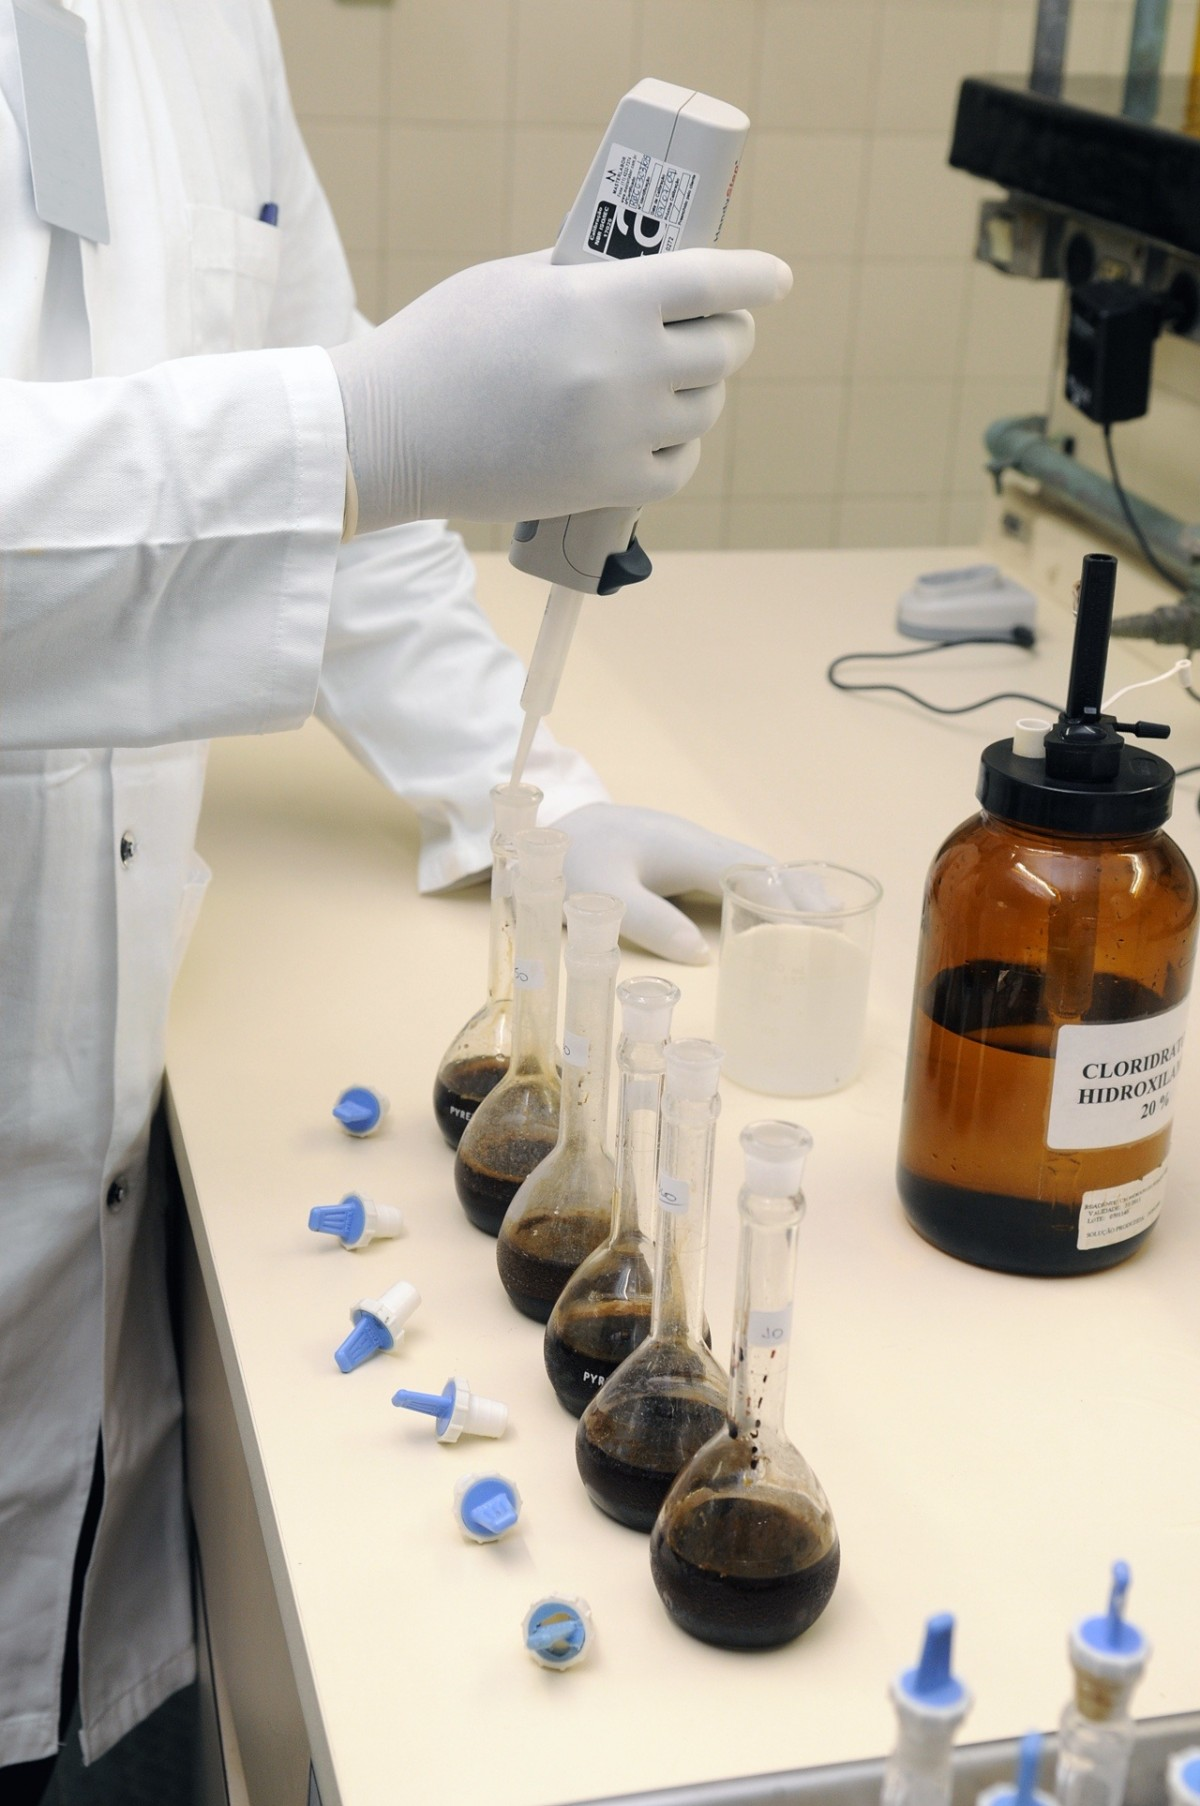
\includegraphics[height=0.75\textheight]{chemist}
    \end{column}
  \end{columns}

\end{Frame}

\begin{frame}[fragile]{Формулы}
  \framesubtitle{Синтаксис}

  \begin{columns}
    \begin{column}{0.25\textwidth}
      \begin{minted}[gobble=8]{salt}
        my_state_id1:
          states_module1.function1
          states_module2.function2:
            - name: overrided_id
            - arg1: value
            - arg2:
                - value1
                - value2
                - value3

        my_state_id2:
          states_module1.function1
      \end{minted}
    \end{column}
    \begin{column}{0.65\textwidth}
      \onslide<+->
      \begin{itemize}[<+-| alert@ +>]
        \footnotesize
        \item Функции состояний принимают аргумент \texttt{name}
        \baselinespace{}
        \item \texttt{name} по умолчанию равен идентификатору
        \baselinespace{}
        \item В формуле может быть множество состояний
        \baselinespace{}
        \item В состоянии можно обращаться к нескольким разным модулям
        \baselinespace{}
        \item В состоянии нельзя обращаться к одному модулю несколько раз
      \end{itemize}
    \end{column}
  \end{columns}
\end{frame}

\begin{frame}{Формулы}
  \framesubtitle{Синтаксис}
  \centering
  \Large
  \inlineicon{\faBomb}Часто можно сделать одно разными путями\\
  \baselinespace{}
  \pause{}
  \inlineicon{\faLightbulb} Хорошо выбрать один способ и придерживаться его
\end{frame}

\begin{Frame}{Модули состояния}
  \begin{itemize}[<+-| alert@ +>]
    \item \texttt{test, saltutil}
    \item \texttt{file, pkg, service, system, \bfseries{cmd}\dots}
    \item \texttt{apache, postgres\_*, redismod\dots}
    \item \texttt{ansiblegate, chef}
  \end{itemize}

  \vfill

  \centering
  \onslide<+->
  Всего на сегодня 349 штук согласно документации
  \only<.>{\overlaypic{south east}{width=100pt}{peaks}}
\end{Frame}

\liveframe{}

\begin{Frame}{Порядок разбора}
  \begin{enumerate}[<+-| alert@ +>]
    \item[0] Разбор на миньоне
    \baselinespace{}
    \item Рендеринг (\texttt{jinja | yaml})
    \baselinespace{}
    \item Определение порядка исполнения
    \baselinespace{}
    \item Исполнение
  \end{enumerate}
  \baselinespace{}

  \centering

  \onslide<+->
  \inlineicon{\faExclamationTriangle} При ошибке на любом этапе --- ответ в шину
\end{Frame}

\begin{Frame}{Порядок исполнения}
  \framesubtitle{Варианты}

  Три пути:
  \vfill
  \begin{enumerate}[<+-| alert@ +>]
    \item В лексикографическом порядке \ExampleIcon{}
    \vfill
    \item По флагу \texttt{order} \ExampleIcon{}
    \vfill
    \item По реквизитам \ExampleIcon{}
  \end{enumerate}

  \centering
  \vfill
  \onslide<+->
  \inlineicon{\faStickyNote} Документация призывает выбрать один способ, и
  следовать ему

  \vfill
\end{Frame}

\begin{frame}{Порядок исполнения}
  \framesubtitle{Предупреждение}
  \begin{center}
    
\includegraphics[height=0.6\textheight]{mess}\\
    \inlineicon{\faRecycle} Реквизиты позволяют элегантно запутать ваш код
      \inlineicon{\faBug}
  \end{center}
\end{frame}

\liveframe{}

\Setsubsection{Каверзы YAML}
\begin{frame}[fragile]
  \frametitle{\Insertsubsection}

  \begin{itemize}[<+-| alert@ +>]
    \item[{\faFrown[regular]}] Стандарт регламентирует использование пробелов
    \item[{\faCheckCircle[regular]}] Не используйте табы

    \vfill

    \item[{\faFrown[regular]}] Вложенный словарь проигнорирован
    \item[{\faCheckCircle[regular]}] Увеличивать отступ
  \end{itemize}

  \vfill

  \begin{columns}
    \begin{column}{0.3\textwidth}
     \onslide<3->
      \begin{minted}[gobble=8]{yaml}
        tree:
          - branch1:
            leaf1: yellow
            leaf2: green
          - branch2:
            leaf1: yellow
      \end{minted}
    \end{column}

    \begin{column}{0.3\textwidth}
      \onslide<4->
      \begin{minted}[gobble=8]{yaml}
        tree:
          - branch:
              leaf1: yellow
              leaf2: green
          - branch:
              leaf1: yellow
      \end{minted}
    \end{column}
  \end{columns}

\end{frame}

\begin{frame}{Каверзы YAML}
  \begin{itemize}[<+-| alert@ +>]
    \item[{\faFrown[regular]}] \texttt{Yes, yes, No, no} и т.~д. грузятся
      как буль
    \item[{\faCheckCircle[regular]}] Оборачивать кавычками

    \vfill

    \item[{\faFrown[regular]}] По стандарту только ASCII
    \item[{\faCheckCircle[regular]}] Стараться использовать ASCII, не вставлять emoji
      \faSmile[regular]
  \end{itemize}
\end{frame}

\begin{frame}{Каверзы YAML}
  \begin{itemize}[<+-| alert@ +>]
    \item[{\faFrown[regular]}] Строки с датой приводятся к \texttt{datetime}, а с
      временем --- к целым
    \item[{\faCheckCircle[regular]}] Оборачивать кавычками

    \vfill

    \item[{\faFrown[regular]}] Символ \texttt{\%} имеет специальное значение, символ
      \texttt{\_} игнорируется в целочисленных литералах
    \item[{\faCheckCircle[regular]}] Кавычки
  \end{itemize}
\end{frame}

\begin{Frame}[c]{Полезные ссылки}
  \setbeamertemplate{itemize items}[square]
  \begin{itemize}
    \setbeamertemplate{itemize item}{\faLink}
    \item[\faBook]
      \uhref{https://docs.saltproject.io/en/latest/contents.html}{%
      Генерируемая документация} (можно скачать \faDownload)
    \item[\faGithub] Когда что-то не работает, наперёд шерст\'им
      \uhref{https://github.com/saltstack/salt/issues}{тикеты на GitHub}
  \end{itemize}
\end{Frame}


\subtitlepage{Jinja}{Шаблонизация формул}

\begin{Frame}[c]{Минутка истории}
  \overlaypic{south east}{width=75pt}{jinja-logo}

  \begin{centering}
    \huge
    Дзиндзя — синтоистский храм
    \footnote{Потому что temple созвучно с template}\\
  \end{centering}

  \vfill

  \begin{itemize}[<+-| @alert ->]
    \item Синтаксис шаблонизатора
      \href{https://www.djangoproject.com/}{Django}, больше возможностей
    \item На Python и для Python
    \item Поддерживает расширения
  \end{itemize}
\end{Frame}

\begin{Frame}[t]{Причины использовать шаблонизатор}
  \overlaypic{south east}{width=80pt}{thumbsup}
  \begin{itemize}[<+-| alert@ +>]
    \item Уменьшается дублирование кода
    \item Доступны grains, pillars, любые внешние данные
    \item Гибкость: условное включение кода
  \end{itemize}
\end{Frame}

\begin{Frame}[c]{Причины НЕ использовать шаблонизатор}
  \centering
  \overlaypic{south east}{width=80pt}{thumbsdown}

  \only<+->{%
    { \huge \bfseries СЛОЖНО\\ }
    Очень легко написать запутанный
    неподдерживаемый код\footnote<2>{Как и в случае с зависимостями}
  }

\end{Frame}

\Setsubsection{Синтаксис}
\begin{frame}[fragile]
  \frametitle{\Insertsubsection}
  \framesubtitle{Окружения}

  \begin{columns}
    \begin{column}{0.40\textwidth}
      \begin{itemize}[<+-| @alert ->]
        \item \texttt{\{\{ \}\}} --- выводимая инструкция \baselinespace{}
        \item \texttt{\{\% \%\}} --- блок [Jinja-кода] \baselinespace{}
        \item \texttt{\{{\# \#}\}} --- комментарий
      \end{itemize}
    \end{column}
    \begin{column}{0.55\textwidth}
      \begin{minted}[gobble=8, linenos=false, frame=lines]{jinja}
        <ul>
        
          {# Этот текст будет удалён шаблонизатором #}
          <li>{{ s }}</li>
        
        </ul>
      \end{minted}
    \end{column}
  \end{columns}

  \vfill

  \onslide<+->
\end{frame}

\begin{frame}{Синтаксис}
  \framesubtitle{Подрезка пробелов}
   \begin{itemize}[<+-| alert@ +>]
     \item[\faCut] Минусы убирают пробельные символы при подстановке
     \item[{\faArrowAltCircleLeft[regular]}] \texttt{\{\%- КОД\_JINJA \%\}} ---
       подрезаются символы слева
     \item[{\faArrowAltCircleRight[regular]}] \texttt{\{\% КОД\_JINJA -\%\}}
       --- подрезаются символы справа
     \item[\faParagraph] \texttt{'\textbackslash{}n'} --- это тоже пробельный
       символ
     \item[\faBan] Плюсы отменяют подрезку, указанную в конфиге шаблонизатора
   \end{itemize}
\end{frame}

\begin{frame}[fragile]
  \frametitle{\Insertsubsection}
  \framesubtitle{Инструкции}

  \setminted{linenos=false, frame=none}

  \begin{itemize}[<+-| @alert ->]
    \item Переменные\\
      \begin{minted}[gobble=8]{jinja}
        
      \end{minted}
    \item Цикл for
      \begin{minted}[gobble=8]{jinja}
        
        {{ i }}
        
      \end{minted}
    \item Условный оператор
      \begin{minted}[gobble=8]{jinja}
         Правда взаправду правда  Неправда 
      \end{minted}
    \item Фильтры и конвееры
      \begin{minted}[gobble=8]{jinja}
        {{ ['соль', 'мука', 'шаблонизатор'] | join(', ') | capitalize }}
      \end{minted}
  \end{itemize}
\end{frame}

\begin{frame}{Синтаксис}
  \framesubtitle{Макросы}

  \overlaypic{south east}{width=75pt}{books}

  \centering
  \inlineicon{\faFire}
  А ещё есть макросы --- это как процедуры\pause,\\
  но мы их пропустим.
\end{frame}

\Setsubsection{Рендеринг произвольного файла}
\begin{frame}[t, fragile]
  \ExampleNote{}

  \frametitle{\Insertsubsection}
  \begin{minted}[gobble=4]{py}
    import jinja2

    filename = 'template.txt'

    with open(filename, 'r') as f:
        template = jinja2.Template(f.read())

    print(template.render())
  \end{minted}
\end{frame}

\begin{Frame}[c]{Jinja и SaltStack}
  \begin{itemize}[<+-| @alert ->]
    \item[\faCube] Jinja подключается как text renderer \vfill
    \item[\faCube] Jinja используется по умолчанию \vfill
    \item[\faCube] Доступны специфичные для SaltStack словари (\texttt{grains},
      \texttt{pillars}) и специальный объект \texttt{salt}
  \end{itemize}
\end{Frame}

\begin{Frame}[t]{Jinja в формулах}
  \ExampleNote{}

  \inputminted[firstnumber=1, firstline=5,]{salt}{../srv/salt/jinja_sample.sls}
  $\nearrow$\footnote{Есть salt.states.win\_powercfg, но раньше он падал
  (\href{https://github.com/saltstack/salt/issues/57393}{\#57393})}

  \vfill{}

  \scriptsize
  \inlineicon{\faCubes} \pause{} \texttt{salt-call slsutil.renderer
  <путь-к-файлу>} чтобы отрендерить формулу.
\end{Frame}

\begin{frame}[t]{Jinja в формулах}
  \ExampleNote{}

  \framesubtitle{Pillar}
  \inputminted[firstnumber=1, firstline=5]{salt}{%
    ../srv/salt/jinja_pillar_sample.sls}

  \vfill{}

  \scriptsize
  \inlineicon{\faCubes} \texttt{salt-call saltutil.refresh\_pillar}
  чтобы синхронизировать пиллары.
\end{frame}

\begin{frame}[c]{Полезные ссылки}
  \setbeamertemplate{itemize items}[square]
  \begin{itemize}
    \item[\faLink] \uhref{https://jinja.palletsprojects.com/}{Документация Jinja}
    \item[\faLink] \uhref{%
        https://docs.saltproject.io/en/latest/topics/jinja/index.html
      }{Раздел документации SaltStack про Jinja}
  \end{itemize}
\end{frame}


\subtitlepage{SaltStack}{Ещё кое-что}

\begin{Frame}{Пишем модули}
  \framesubtitle{Особенности}

  \begin{center}
    Все мы в душ\'е немного программисты \inlineicon{\faKeyboard[regular]}
  \end{center}

  \onslide<+->

  \begin{itemize}[<+-| alert@ +>]
    \setbeamertemplate{itemize item}{\faCode}

    \item[\faPython] Python\vfill
    \item[{\faHandshake[regular]}] Единые соглашения для разных модулей\vfill
    \item[\faHatWizard] Различающийся контекст
    \item[\faMicroscope] Работает через интроспекцию
    \item[\faSkullCrossbones] Аннотирование типов ломает интроспекцию
  \end{itemize}

  \vfill

  \onslide<+->
  \begin{center}
    \inlineicon{\faLightbulb[regular]}
    Не забываем \texttt{salt '*' saltutil.sync\_all}
  \end{center}

  \overlaypic{south east}{width=75pt}{snake}
\end{Frame}

\begin{frame}{Пишем модули}
  \framesubtitle{Соглашения}

  \ExampleNote{}

  \begin{itemize}[<+-| alert@ +>]
    \setbeamertemplate{itemize item}{\faCode}
    \item Ищутся любые подходящие функции
    \item Функции возвращают словари
    \item \texttt{\_\_virtual\_\_: function}
    \item \texttt{\_\_init\_\_: function}, получающая настройки миньона
    \item \texttt{\_\_salt\_\_: dict}\footnote{%
      На деле \texttt{NamedLoaderContext} \faGhost}
    \item \texttt{\_\_virtualname\_\_: str}
    \item \texttt{\_\_func\_alias\_\_: dict}
  \end{itemize}
\end{frame}

\liveframe{}

\begin{Frame}{Реакторы}

  \ExampleNote{}

  \begin{itemize}[<+-| alert@ +>]
    \item Действие по событию (как callback)
    \item Прописываются последовательностью в конфиге мастера
    \item Сопоставляют действие тэгу события
    \item Бывают local, runner, wheel и caller
    \item Переменные Jinja доступны ограниченно, реквизитов нет
    \item[\faTerminal] \texttt{salt-run event.send ТЭГ СЛОВАРЬ} для отладки
  \end{itemize}

  \vfill

  \centering
  
\includegraphics[width=75pt]{iso-radiation}
\end{Frame}

\liveframe{}

\Setsubsection{Шедулинг}
\begin{frame}[fragile]
  \frametitle{\Insertsubsection}

  \begin{itemize}[<+-| alert@ +>]
    \setbeamertemplate{itemize items}{\faClock[regular]}

    \item Похоже на cron или systemd.timer
    \item Прописывается в конфиге миньона или мастера
    \item Запуск модулей, применение состояний
    \item На миньоне модули исполнения, на мастере модули раннеров
  \end{itemize}

  \onslide<+->
  \begin{center}\begin{minipage}{0.4\textwidth}
    \begin{minted}[gobble=6]{yaml}
      schedule:
        write_to_file:
          function: cmd.run
          seconds: 5
          args:
            - 'date >> /tmp/salt.log'
          kwargs: {}
          splay: 3
    \end{minted}
  \end{minipage}\end{center}
\end{frame}

\liveframe{}

\begin{Frame}{В двух словах о Salt Mine}
  \begin{itemize}[<+-| alert@ +>]
    \item Шахты похожи на грейны
    \item Значения доступны для миньонов
    \item Можно настроить в конфиге миньона
    \item Можно настроить в пилларах
    \item Для получения значений \texttt{mine.get}
    \item[\faAngleDoubleRight] Пример в следующей секции
  \end{itemize}
\end{Frame}

\begin{Frame}{Оркестрация}
  \framesubtitle{Это\dots}

  \ExampleNote{}

  \begin{itemize}[<+-| alert@ +>]
    \item[\faRunning] Salt Orchestration Runner
    \item[\faMountain] Выше, чем highstate
    \item[\faBullhorn] Вызовы функций для управления инфраструктурой
    \item[\faTerminal] \texttt{salt-run state.orchestrate SLS\_ФАЙЛ}
  \end{itemize}
\end{Frame}

\begin{frame}{Оркестрация}
  \framesubtitle{Матрёшка}
  \centering
  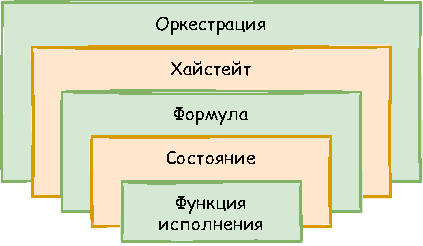
\includegraphics[width=0.5\textwidth]{saltstack-matryoshka}
  \overlaypic{south east}{width=140pt}{matryoshkas}
\end{frame}

\liveframe{}

\begin{Frame}{Salt Cloud}
  \begin{itemize}[<+-| alert@ +>]
    \item[\faCloud] Провиженинг виртуальных машин
    \item[\faCogs] Куча коннекторов\footnote<2->{Но не для отечественных
      \faCloud\faCloud\faMeh[regular]}
    \item[{\faFileCode[regular]}] Определяем провайдера и профиль машины
    \item[\faServer] Элегантно разворачиваемся
    \item[{\faMap[regular]}] mapfile для подхода <<инфраструктура как код>>
  \end{itemize}
\end{Frame}

\begin{frame}{Salt Cloud}
  \framesubtitle{Команда}

  \ExampleNote{}

  \setbeamertemplate{itemize item}{\faTerminal}

  \begin{itemize}[<+->]
    \item \texttt{salt-cloud [-P] -p ПРОФИЛЬ ИМЯ\_1 ИМЯ\_2 \ldots\ ИМЯ\_N} \\
      \color{Gray} \small Создать машины из профиля (\texttt{-P} --- параллельно)

    \vfill

    \item \texttt{salt-cloud [-P] -m МАПФАЙЛ} \\
      \color{Gray} \small Создать машины по карте

    \vfill

    \item \texttt{salt-cloud -m МАПФАЙЛ -d} \\
      \color{Gray} \small Удалить машины, указанные в карте

  \end{itemize}
\end{frame}

\liveframe{}

\begin{Frame}{Ссылки на документацию}

  \vfill
  \begin{itemize}
    \setbeamertemplate{itemize item}{\faLink}
    \item \uhref{%
      https://docs.saltproject.io/en/latest/topics/development/modules/developing.html}{%
      Разработка модулей}\vfill

    \item \uhref{%
      https://docs.saltproject.io/en/latest/topics/reactor/index.html}{%
      Реакторы}\vfill

    \item \uhref{%
      https://docs.saltproject.io/en/latest/topics/jobs/index.html\#scheduling-jobs}{%
      Планируемые задачи}\vfill

    \item \uhref{%
      https://docs.saltproject.io/en/latest/topics/orchestrate/orchestrate_runner.html}{%
      Оркестрация}\vfill

    \item \uhref{%
      https://docs.saltproject.io/en/latest/topics/cloud/index.html}{%
      Salt Cloud}\vfill
  \end{itemize}
\end{Frame}

% vi: ft=tex


\section{Заключение}
\begin{custom-bg-frame}{toad}
\end{custom-bg-frame}

\begin{bg-frame}
  \vspace{2.0\baselineskip}
  {\huge Спасибо за внимание!}\\
  \rule{180pt}{\rulewidth}\\
  \insertauthor{} \insertcontacts{}\\
  \vspace{0.25\baselineskip}
  \inserthomepage{}
\end{bg-frame}

\end{document}
